% answers.tex —— 2008 年·全国大纲卷Ⅱ·文科 · 参考答案与详细解析片段
% 由 tools/generate_projects.py 依来源总账自 2008/2008_数学真题_全国2文_试题.md + 2008/2008_数学真题_全国2文_解析正文.md + 2008/2008_数学真题_全国2文_答案要点.md 生成，勿手改（改源 MD 后重跑）


\begin{gktip}
固定源 PDF 为印刷页码 439–440 的两页题面，不附答案。以下解析均依据固定源独立复算；第 20 题图形在 LaTeX 工程中以 TikZ/PGFPlots 矢量源重绘。
\end{gktip}

\begin{answer}
\gksolhead{1}{}

\textbf{题目}：

若 $\sin\alpha<0$ 且 $\tan\alpha>0$，则 $\alpha$ 是\mbox{（　　）}

（A）第一象限角\quad（B）第二象限角\quad（C）第三象限角\quad（D）第四象限角

\Needspace{4\baselineskip}
\textbf{解析}

$\sin\alpha<0$ 且 $\tan\alpha>0$ 表明 $\cos\alpha<0$，故 $\alpha$ 在第三象限，选 C。

\gkanswer{答案：C}

\end{answer}
\begin{answer}
\gksolhead{2}{}

\textbf{题目}：

设集合 $M=\{m\in\mathbb Z\mid-3<m<2\}$，$N=\{n\in\mathbb Z\mid-1\leqslant n\leqslant3\}$，则 $M\cap N=$\mbox{（　　）}

（A）$\{0,1\}$\quad（B）$\{-1,0,1\}$\quad（C）$\{0,1,2\}$\quad（D）$\{-1,0,1,2\}$

\Needspace{4\baselineskip}
\textbf{解析}

$M=\{-2,-1,0,1\}$，$N=\{-1,0,1,2,3\}$，故交集为 $\{-1,0,1\}$，选 B。

\gkanswer{答案：B}

\end{answer}
\begin{answer}
\gksolhead{3}{}

\textbf{题目}：

原点到直线 $x+2y-5=0$ 的距离为\mbox{（　　）}

（A）$1$\quad（B）$\sqrt3$\quad（C）$2$\quad（D）$\sqrt5$

\Needspace{4\baselineskip}
\textbf{解析}

\Needspace{5\baselineskip}
原点到直线的距离为

\nopagebreak[4]
\[
\frac5{\sqrt{1^2+2^2}}=\sqrt5
\]

选 D。

\gkanswer{答案：D}

\end{answer}
\begin{answer}
\gksolhead{4}{}

\textbf{题目}：

函数 $f(x)=\dfrac1x-x$ 的图象关于\mbox{（　　）}

（A）$y$ 轴对称\quad（B）直线 $y=-x$ 对称\quad（C）坐标原点对称\quad（D）直线 $y=x$ 对称

\Needspace{4\baselineskip}
\textbf{解析}

$f(-x)=-1/x+x=-f(x)$，故图象关于原点对称，选 C。

\gkanswer{答案：C}

\end{answer}
\begin{answer}
\gksolhead{5}{}

\textbf{题目}：

若 $x\in(e^{-1},1)$，$a=\ln x$，$b=2\ln x$，$c=\ln^3x$，则\mbox{（　　）}

（A）$a<b<c$\quad（B）$c<a<b$\quad（C）$b<a<c$\quad（D）$b<c<a$

\Needspace{4\baselineskip}
\textbf{解析}

令 $t=\ln x\in(-1,0)$，则 $a=t,b=2t,c=t^3$，比较负数大小得 $b<c<a$，选 D。

\gkanswer{答案：D}

\end{answer}
\begin{answer}
\gksolhead{6}{}

\textbf{题目}：

\Needspace{5\baselineskip}
设变量 $x,y$ 满足约束条件

\nopagebreak[4]
\[
\begin{cases}
y\geqslant x,\\
x+2y\leqslant2,\\
x\geqslant-2,
\end{cases}
\]

则 $z=x-3y$ 的最小值为\mbox{（　　）}

（A）$-2$\quad（B）$-4$\quad（C）$-6$\quad（D）$-8$

\Needspace{4\baselineskip}
\textbf{解析}

\Needspace{5\baselineskip}
目标函数在固定 $x$ 时随 $y$ 增大而减小，取上边界 $y=1-x/2$，得

\nopagebreak[4]
\[
z=x-3\left(1-\frac x2\right)=\frac52x-3
\]

在 $x\geqslant-2$ 的可行范围内最小值在 $x=-2$ 处取得，为 $-8$，选 D。

\gkanswer{答案：D}

\end{answer}
\begin{answer}
\gksolhead{7}{}

\textbf{题目}：

设曲线 $y=ax^2$ 在点 $(1,a)$ 处的切线与直线 $2x-y-6=0$ 平行，则 $a=$\mbox{（　　）}

（A）$1$\quad（B）$\dfrac12$\quad（C）$-\dfrac12$\quad（D）$-1$

\Needspace{4\baselineskip}
\textbf{解析}

曲线在 $x=1$ 处的切线斜率为 $2a$，给定直线斜率为 $2$，故 $a=1$，选 A。

\gkanswer{答案：A}

\end{answer}
\begin{answer}
\gksolhead{8}{}

\textbf{题目}：

正四棱锥的侧棱长为 $2\sqrt3$，侧棱与底面所成的角为 $60^\circ$，则该棱锥的体积为\mbox{（　　）}

（A）$3$\quad（B）$6$\quad（C）$9$\quad（D）$18$

\Needspace{4\baselineskip}
\textbf{解析}

\Needspace{5\baselineskip}
侧棱与底面成 $60^\circ$，故棱锥高为 $2\sqrt3\sin60^\circ=3$。设底面边长为 $s$，由侧棱的水平投影得

\nopagebreak[4]
\[
\left(\frac{s}{\sqrt2}\right)^2=(2\sqrt3)^2-3^2=3
\]

故底面面积为 $s^2=6$，体积为 $6$，选 B。

\gkanswer{答案：B}

\end{answer}
\begin{answer}
\gksolhead{9}{}

\textbf{题目}：

$(1-\sqrt{x})^4(1+\sqrt{x})^4$ 的展开式中 $x$ 的系数是\mbox{（　　）}

（A）$-4$\quad（B）$-3$\quad（C）$3$\quad（D）$4$

\Needspace{4\baselineskip}
\textbf{解析}

\nopagebreak[4]
\[
(1-\sqrt x)^4(1+\sqrt x)^4=(1-x)^4
\]

$x$ 的系数为 $-4$，选 A。

\gkanswer{答案：A}

\end{answer}
\begin{answer}
\gksolhead{10}{}

\textbf{题目}：

函数 $f(x)=\sin x-\cos x$ 的最大值为\mbox{（　　）}

（A）$1$\quad（B）$\sqrt2$\quad（C）$\sqrt3$\quad（D）$2$

\Needspace{4\baselineskip}
\textbf{解析}

\nopagebreak[4]
\[
\sin x-\cos x=\sqrt2\sin\left(x-\frac\pi4\right)
\]

最大值为 $\sqrt2$，选 B。

\gkanswer{答案：B}

\end{answer}
\begin{answer}
\gksolhead{11}{}

\textbf{题目}：

设 $\triangle ABC$ 是等腰三角形，$\angle ABC=120^\circ$，则以 $A\text{、}B$ 为焦点且过点 $C$ 的双曲线的离心率为\mbox{（　　）}

（A）$\dfrac{1+\sqrt2}{2}$\quad（B）$\dfrac{1+\sqrt3}{2}$\quad（C）$1+\sqrt2$\quad（D）$1+\sqrt3$

\Needspace{4\baselineskip}
\textbf{解析}

\Needspace{5\baselineskip}
等腰三角形中 $BA=BC$，且 $\angle ABC=120^\circ$，故 $AC=\sqrt3\,AB$。以 $A,B$ 为焦点的双曲线经过 $C$，有 $2a=AC-BC=(\sqrt3-1)AB$，$2c=AB$，所以

\nopagebreak[4]
\[
e=\frac1{\sqrt3-1}=\frac{1+\sqrt3}{2}
\]

选 B。

\gkanswer{答案：B}

\end{answer}
\begin{answer}
\gksolhead{12}{}

\textbf{题目}：

已知球的半径为 $2$，相互垂直的两个平面分别截球面得两个圆。若两圆的公共弦长为 $2$，则两圆的圆心距等于\mbox{（　　）}

（A）$1$\quad（B）$\sqrt2$\quad（C）$\sqrt3$\quad（D）$2$

\Needspace{4\baselineskip}
\textbf{解析}

\Needspace{5\baselineskip}
设两平面到球心的距离为 $d_1,d_2$。公共弦长为 $2$ 给出

\nopagebreak[4]
\[
2\sqrt{4-d_1^2-d_2^2}=2
\]

故 $d_1^2+d_2^2=3$，这正是两圆圆心距的平方，圆心距为 $\sqrt3$，选 C。

\gkanswer{答案：C}

\end{answer}
\begin{answer}
\gksolhead{13}{}

\textbf{题目}：

设向量 $\boldsymbol a=(1,2)$，$\boldsymbol b=(2,3)$。若向量 $\lambda\boldsymbol a+\boldsymbol b$ 与向量 $\boldsymbol c=(-4,-7)$ 共线，则 $\lambda=$\gkblank{}。

\Needspace{4\baselineskip}
\textbf{解析}

\Needspace{5\baselineskip}
共线条件为

\nopagebreak[4]
\[
\begin{vmatrix}\lambda+2&2\lambda+3\\-4&-7\end{vmatrix}=0
\]

解得 $\lambda=2$。

\gkanswer{答案：$2$}

\end{answer}
\begin{answer}
\gksolhead{14}{}

\textbf{题目}：

从 $10$ 名男同学、$6$ 名女同学中选 $3$ 名参加体能测试，则选到的 $3$ 名同学中既有男同学又有女同学的不同选法共有\gkblank{}种。（用数字作答）

\Needspace{4\baselineskip}
\textbf{解析}

\Needspace{5\baselineskip}
总选法为 $\binom{16}{3}$，减去全男和全女：

\nopagebreak[4]
\[
\binom{16}{3}-\binom{10}{3}-\binom63=560-120-20=420
\]

\gkanswer{答案：$420$}

\end{answer}
\begin{answer}
\gksolhead{15}{}

\textbf{题目}：

已知 $F$ 是抛物线 $C:y^2=4x$ 的焦点，$A\text{、}B$ 是 $C$ 上的两个点，线段 $AB$ 的中点为 $M(2,2)$，则 $\triangle ABF$ 的面积等于\gkblank{}。

\Needspace{4\baselineskip}
\textbf{解析}

抛物线参数方程取 $P(t)=(t^2,2t)$。设两端参数为 $t_1,t_2$，中点条件给出 $t_1+t_2=2$、$t_1^2+t_2^2=4$，从而 $t_1t_2=0$。两端点为 $(0,0),(4,4)$，焦点为 $(1,0)$，三角形面积为 $2$。

\gkanswer{答案：$2$}

\end{answer}
\begin{answer}
\gksolhead{16}{}

\textbf{题目}：

平面内的一个四边形为平行四边形的充要条件有多个，如两组对边分别平行。类似地，写出空间中的一个四棱柱为平行六面体的两个充要条件：充要条件①\gkblank{}；充要条件②\gkblank{}。（写出你认为正确的两个充要条件）

\Needspace{4\baselineskip}
\textbf{解析}

例如可取两个充要条件：两个底面都是平行四边形；任意两个相邻侧面均为平行四边形。它们分别保证底面两组边和侧棱方向形成三组平行线，从而得到平行六面体。

\gkanswer{答案：两组相对的侧面分别为平行四边形；两个底面都是平行四边形。}

\end{answer}
\begin{answer}
\gksolhead{17}{}

\textbf{题目}：

在 $\triangle ABC$ 中，$\cos A=-\dfrac5{13}$，$\cos B=\dfrac35$。

（1） 求 $\sin C$ 的值；

（2） 设 $BC=5$，求 $\triangle ABC$ 的面积。

\Needspace{4\baselineskip}
\textbf{解析}

\gksubpart{(1)}

\Needspace{5\baselineskip}
$\sin A=12/13$，$\sin B=4/5$，故

\nopagebreak[4]
\[
\sin C=\sin(A+B)=\sin A\cos B+\cos A\sin B
=\frac{12}{13}\cdot\frac35-\frac5{13}\cdot\frac45
=\frac{16}{65}
\]

\gksubpart{(2)}

\Needspace{5\baselineskip}
由正弦定理，边长比例为 $a:b:c=15:13:4$。因 $BC=a=5$，可得 $b=13/3$，从而

\nopagebreak[4]
\[
S=\frac12\cdot5\cdot\frac{13}{3}\cdot\frac{16}{65}
=\frac83
\]

\gkanswer{答案（1）：$\sin C=\dfrac{16}{65}$。}

\gkanswer{答案（2）：$\triangle ABC$ 的面积为 $\dfrac83$。}

\end{answer}
\begin{answer}
\gksolhead{18}{}

\textbf{题目}：

等差数列 $\{a_n\}$ 中，$a_4=10$，且 $a_3\text{、}a_6\text{、}a_{10}$ 成等比数列。求数列 $\{a_n\}$ 前 $20$ 项的和 $S_{20}$。

\Needspace{4\baselineskip}
\textbf{解析}

\Needspace{5\baselineskip}
设等差数列首项为 $a_1$，公差为 $d$。由 $a_4=10$，有 $a_3=10-d,a_6=10+2d,a_{10}=10+6d$。等比条件给出

\nopagebreak[4]
\[
(10+2d)^2=(10-d)(10+6d)
\]

即 $d(d-1)=0$。因此 $d=0$ 或 $d=1$，相应 $S_{20}=200$ 或 $330$。若原题隐含要求非等差常数列，应取 $d=1$；固定源题面未见该限制，故保留两解并记待核。

\gkanswer{答案：$S_{20}=200$ 或 $330$（等差数列公差分别为 $0$ 或 $1$，题面未排除公差为零）。}

\end{answer}
\begin{answer}
\gksolhead{19}{}

\textbf{题目}：

甲、乙两人进行射击比赛，在一轮比赛中，甲、乙各射击一发子弹。根据以往资料知，甲击中 $8$ 环、$9$ 环、$10$ 环的概率分别为 $0.6,0.3,0.1$，乙击中 $8$ 环、$9$ 环、$10$ 环的概率分别为 $0.4,0.4,0.2$。设甲、乙的射击相互独立。

（1） 求在一轮比赛中甲击中的环数多于乙击中环数的概率；

（2） 求在独立的三轮比赛中，至少有两轮甲击中的环数多于乙击中环数的概率。

\Needspace{4\baselineskip}
\textbf{解析}

\gksubpart{(1)}

\Needspace{5\baselineskip}
单轮甲胜出的概率为

\nopagebreak[4]
\[
p=0.6(0)+0.3(0.4)+0.1(0.4+0.4)=0.2
\]

\gksubpart{(2)}

\Needspace{5\baselineskip}
三轮中至少两轮胜出的概率为

\nopagebreak[4]
\[
\binom32p^2(1-p)+p^3
=3\left(\frac15\right)^2\frac45+\left(\frac15\right)^3
=\frac{13}{125}
\]

\gkanswer{答案（1）：$\dfrac15$。}

\gkanswer{答案（2）：$\dfrac{13}{125}$。}

\end{answer}
\begin{answer}
\gksolhead{20}{}

\textbf{题目}：

如图，正四棱柱 $ABCD-A_1B_1C_1D_1$ 中，$AA_1=2AB=4$，点 $E$ 在 $CC_1$ 上且 $C_1E=3EC$。
\nopagebreak[4]
\begin{center}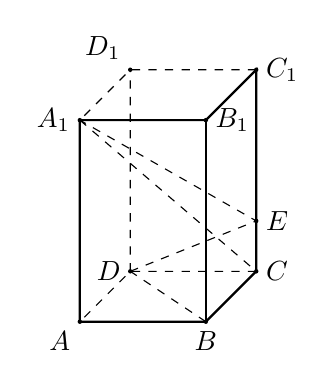
\begin{tikzpicture}[scale=.8,>=stealth]
\coordinate (A) at (0,0); \coordinate (B) at (2,0);
\coordinate (C) at (2.8,.8); \coordinate (D) at (.8,.8);
\coordinate (A1) at (0,3.2); \coordinate (B1) at (2,3.2);
\coordinate (C1) at (2.8,4); \coordinate (D1) at (.8,4);
\coordinate (E) at (2.8,1.6);
\draw[thick] (A)--(B)--(C)--(C1)--(B1)--(A1)--cycle;
\draw[dashed] (C)--(D)--(A) (C1)--(D1)--(A1) (D)--(D1);
\draw[thick] (B)--(B1) (C)--(C1);
\draw[dashed] (A1)--(C) (B)--(D) (D)--(E)--(A1);
\fill (A) circle (1pt) node[below left] {$A$};
\fill (B) circle (1pt) node[below] {$B$};
\fill (C) circle (1pt) node[right] {$C$};
\fill (D) circle (1pt) node[left] {$D$};
\fill (A1) circle (1pt) node[left] {$A_1$};
\fill (B1) circle (1pt) node[right] {$B_1$};
\fill (C1) circle (1pt) node[right] {$C_1$};
\fill (D1) circle (1pt) node[above left] {$D_1$};
\fill (E) circle (1pt) node[right] {$E$};
\end{tikzpicture}
\end{center}
\nopagebreak[4]
（1） 证明：$A_1C\perp$ 平面 $BED$；

（2） 求二面角 $A_1-DE-B$ 的大小。

\Needspace{4\baselineskip}
\textbf{解析}

\gksubpart{(1)}

\Needspace{5\baselineskip}
取 $A=(0,0,0),B=(2,0,0),C=(2,2,0),D=(0,2,0)$，高为 $4$，且 $E=(2,2,1)$。计算

\nopagebreak[4]
\[
\overrightarrow{A_1C}=(2,2,-4),\quad
\overrightarrow{BE}=(0,2,1),\quad
\overrightarrow{BD}=(-2,2,0)
\]

可得 $\overrightarrow{A_1C}$ 同时垂直于 $\overrightarrow{BE}$、$\overrightarrow{BD}$，故垂直于平面 $BED$。

\gksubpart{(2)}

\Needspace{5\baselineskip}
取平面 $A_1DE$ 与 $BDE$ 的法向量，内积计算得二面角余弦为

\nopagebreak[4]
\[
\cos\theta=\frac1{\sqrt{126}}
\]

\gkanswer{答案（1）：见解析版}

\gkanswer{答案（2）：二面角 $A_1-DE-B$ 的余弦为 $\dfrac1{\sqrt{126}}$。}

\end{answer}
\begin{answer}
\gksolhead{21}{}

\textbf{题目}：

设 $a\in\mathbb R$，函数 $f(x)=ax^3-3x^2$。

（1） 若 $x=2$ 是函数 $y=f(x)$ 的极值点，求 $a$ 的值；

（2） 若函数 $g(x)=f(x)+f'(x)$，$x\in[0,2]$，在 $x=0$ 处取得最大值，求 $a$ 的取值范围。

\Needspace{4\baselineskip}
\textbf{解析}

\gksubpart{(1)}

$f'(x)=3ax^2-6x=3x(ax-2)$。$x=2$ 为极值点要求 $f'(2)=0$，故 $a=2$。

\gksubpart{(2)}

\Needspace{5\baselineskip}
此时

\nopagebreak[4]
\[
g(x)=2x^3+3x^2-6x=x(2x^2+3x-6)
\]

要使 $g(x)\leqslant g(0)=0$ 对 $[0,2]$ 成立，只需 $2x^2+3x-6\leqslant0$ 在区间内成立，临界端点条件给出 $a\leqslant6/5$。一般保留参数计算得取值范围为 $a\leqslant6/5$。

\gkanswer{答案（1）：$a=2$。}

\gkanswer{答案（2）：$a\leqslant\dfrac65$。}

\end{answer}
\begin{answer}
\gksolhead{22}{}

\textbf{题目}：

设椭圆中心在坐标原点，$A(2,0)$、$B(0,1)$ 是它的两个顶点，直线 $y=kx$（$k>0$）与 $AB$ 相交于点 $D$，与椭圆相交于 $E\text{、}F$ 两点。

（1） 若 $\overline{ED}=6\overline{DF}$，求 $k$ 的值；

（2） 求四边形 $AEBF$ 面积的最大值。

\Needspace{4\baselineskip}
\textbf{解析}

\gksubpart{(1)}

\Needspace{5\baselineskip}
设直线 $y=kx$ 与椭圆交于横坐标 $\pm r$ 的两点。由向量比例 $\overrightarrow{ED}=6\overrightarrow{DF}$ 得 $D$ 将 $EF$ 按 $1:6$ 分点，代入 $D$ 与 $AB$ 的交点坐标得到

\nopagebreak[4]
\[
24k^2-25k+6=0
\]

故 $k=2/3$ 或 $k=3/8$。

\gksubpart{(2)}

\Needspace{5\baselineskip}
四边形面积等于两条对角线乘积的一半。化简为

\nopagebreak[4]
\[
S(k)=\frac{2(2k+1)}{\sqrt{1+4k^2}}
\]

其最大值在 $k=1/2$ 处取得，最大面积为 $2\sqrt2$。

\gkanswer{答案（1）：$k=\dfrac23$ 或 $k=\dfrac38$。}

\gkanswer{答案（2）：四边形 $AEBF$ 面积的最大值为 $2\sqrt2$。}

\end{answer}